\chapter{Graph Traversals and Applications}
\label{ch:traversal}

Many graph problems require us to visit each node of a digraph in a 
systematic way. For example, we may want to print out the labels of the
nodes in some order, or perhaps we are in a maze and we have
no idea where to find the door. More interesting examples will be
described below. The important requirements are that we must be
systematic (otherwise an algorithm is hard to implement), we must be
complete (visit each node at least once), and we must be efficient
(visit each node at most once). 

There are several ways to perform such a traversal.  Here we present the
two most common, namely breadth-first search and depth-first search.
We also discuss a more general but also more complicated and slower 
algorithm, priority-first search. First we start with general remarks 
applicable to all graph traversals.

\section{Generalities on graph traversal}
\label{sec:trav}

We first discuss a general skeleton common to all graph traversals. In
Figure~\ref{fig:travcode}, this general skeleton is presented in
pseudocode. We first describe it less formally.

\begin{figure}[htbp]
\label{fig:travcode}

\Algorithm{traverse}{digraph $G$}{}
{
array $colour[n]$ array $pred[n]$ \\

\textbf{for} $u \in V(G)$ \textbf{do} \\

\> $colour[u] \gets $ WHITE \\

\textbf{end for}\\

\textbf{for}  $s\in V(G)$ \textbf{do} \\

\> \textbf{if} $colour[s] = $ WHITE \textbf{then} \\

\> \> \texttt{visit}($s$) \\

\> \textbf{end if}\\

\textbf{end for}\\

\textbf{return} $pred$ \\
}


\Algorithm{visit}{node $s$ of digraph $G$}{}
{

$colour[s] \gets $ GREY; $pred[s] \gets $ NULL \\

\textbf{while} there is a grey node \textbf{do} \\

\> choose a grey node $u$ \\

\> \textbf{if} there is a white neighbour of $u$  \\

\> \> choose such a neighbour $v$ \\

\> \> $colour[v] \gets $ GREY; $pred[v] \gets u$ \\

\> \textbf{else} $colour[u] \gets $ BLACK \\

\> \textbf{end if} \\

\textbf{end while}\\
}

\caption{Graph traversal schema}

\end{figure}


Suppose that $G$ is a digraph. Choose a node $v$ as a starting point. We
shall visit all nodes reachable from $v$ in $G$ using an obvious method.

At each stage, there are three possible types of nodes. \defnfont{White}
nodes are those that have not yet been visited. \defnfont{Grey} nodes
are those that have been visited but have adjacent nodes that are white.
Finally, \defnfont{black} nodes are those that nodes that have been
visited, along with all their adjacent nodes. This is shown pictorially in Figure~\ref{fig:travcols}. 

\begin{figure}

FILL IN PICTURE

\caption{Node states in the middle of a digraph traversal}
\label{fig:travcols}

\end{figure}


Initially, all nodes are white. The traversal algorithm first colours
$v$ grey. At each subsequent step, it chooses a grey node $w$ and then a
white node $x$  adjacent to $w$ (thereby changing the colour of $x$ to
grey). This possibly causes some grey nodes to become black. When all
nodes are black, there can be no white nodes reachable from the current
set of visited nodes. We have reached every node that can be reached
from the root, and the traversal from $v$ terminates. 

At this stage we have created a subdigraph of $G$ that is a tree: the
nodes are precisely the black nodes, and the arcs are those arcs
connecting a grey node to its white neighbour at the instant before the
white node turns grey.

There may remain unvisited nodes in the digraph. In this case, we may
choose another white node as root and continue. Eventually, we obtain a
set of disjoint trees spanning the digraph, which we call the
\defnfont{search forest}. 

The above is formalized in Figure~\ref{fig:travcode}. Here \algfont{traverse} simply chooses a new root $s$ when required. The main work is done by \algfont{visit}. In this procedure, the array $pred$ stores the parent of each node; each root gets the value NULL, since it has no parent. Each time through the while-loop, a white node is turned grey or a grey node is turned black. Thus eventually there are no white nodes reachable from $s$ and the procedure terminates. If a node $u$ is reachable from $s$ then it is visited during the call to \algfont{visit} with input $s$, unless it had already been visited in a previous tree.

Now once a traversal has been completed search forest has been obtained, we may classify the arcs into four distinct types. This classification will be very useful later.

\begin{Definition}
Suppose we have performed a traversal of a digraph $G$, resulting in a
search forest $F$.  Let $(u, v)\in E(G)$ be an arc. It is called a
\defnfont{tree} arc if it belongs to one of the trees of $F$. If the arc
is not a tree arc, there are three possibilities.  A non-tree arc is
called a \defnfont{forward} arc if $u$ is an ancestor of $v$ in $F$, a
\defnfont{back} arc if $u$ is a descendant of $v$ in $F$, and a
\defnfont{cross} arc if neither $u$ nor $v$ is an ancestor of the other in $F$.

\end{Definition} 

\begin{note}

In the first three cases above, $u$ and $v$ must belong to the same
tree of $F$. However, a cross arc may join two nodes in the same tree
or point from one tree to another. 

\end{note}

The following theorem collects all the basic facts we need for proofs in later sections. Figure~\ref{fig:travdecomp} illustrates the first part.


\begin{Theorem}
\label{thm:trav}
Suppose that we have carried out \algfont{traverse} on a digraph $G$, resulting in a search forest $F$. Let $v, w \in V(G)$.
\begin{enumerate}
\item Let $T_1$ and $T_2$ be different trees in $F$ and suppose that $T_1$ was explored before $T_2$. Then there are no arcs from $T_1$ to $T_2$. 

\item Suppose that $G$ is a graph. Then there can be no edges joining different trees of $F$.

\item Suppose that $v$ is visited before $w$ and $w$ is reachable from $v$ in $G$. Then $v$ and $w$ belong to the same tree of $F$.

\item Suppose that $v$ and $w$ belong to the same tree $T$ in $F$. Then any path from $v$ to $w$ in $G$ must have all nodes in $T$.

\end{enumerate}
\end{Theorem}

\begin{proof}

If the first part were not true, then since $w$ is reachable from $v$, and $w$ has not been visited before $T_1$ is started, $w$ must be reached in the generation of $T_1$, contradicting $w\in T_2$. The second part follows immediately for symmetric digraphs and hence for graphs. Now suppose that $v$ is seen before $w$. Let $r$ be the root of the tree $T$ containing $v$. Then $w$ is reachable from $r$ and so since it has not already been visited when $r$ is chosen, it belongs to $T$. Finally, if $v$ and $w$ are in the same tree, then any path from $v$ to $w$ in $G$ going outside the tree must re-enter it via some arc; either the leaving or the entering arc will contradict the first part. 
\end{proof}


\begin{figure}[htbp]

\caption{Decomposition of a digraph in terms of search trees}
\label{fig:travdecomp}
\end{figure}

We now turn to the analysis of \algfont{traverse}. The generality
of our traversal procedure makes its complexity hard to determine.  Its
running time is very dependent on how one chooses the next grey node $u$
and its white neighbour $v$. It also apparently depends on how long it
takes to determine whether there exist any grey nodes or whether $u$ has
any white neighbours. However, any sensible rule for checking existence
of either type of node should simply return false if there is no such
node, and take no more time in this case than if it does find one. Thus
we do not need to take account of the checking in our analysis.

Since the initialization of the array $colour$ takes time 
$\Theta(n)$, the time taken by \algfont{traverse} is clearly $\Theta(n +
V)$, where $V$ is the total time taken by all the calls to \algfont{visit}.

Each time through the while-loop of \algfont{visit} a grey node is
chosen, and either a white node is turned grey or a grey node is turned
black. Note that the same grey node can be chosen many times. Thus we
execute the while-loop in total $\Theta(n)$
times since every node must eventually move from white through grey to
black. Let $a, A$ be lower and upper bounds on the time taken to choose a grey node (note that they may depend on $n$ and be quite large if the rule used is not very simple). Then the time taken in choosing grey nodes is $O(An)$ and $\Omega(an)$. Now consider the time taken to find a white neighbour. This will involve examining each  neighbour of $u$ and checking whether it is white, then applying a selection rule. If the time taken to apply the rule is at
least $b$ most $B$ (which may depend on $n$), then the total time in choosing white neighbours is $O(B e)$ and $\Omega(be)$ if adjacency lists are used and $O(Bn^2)$ and $\Omega(bn^2)$ if an adjacency matrix is used.

In summary, then, the running time of \algfont{traverse} is $O(An + Be)$
and $\Omega(an + be)$ if adjacency lists are used, and $O(A n + B n^2)$ and $\Omega(an + bn^2)$ if adjacency matrix format is used.

A more detailed analysis would depend on the rule used. We shall see in
Section~\ref{sec:BFSDFS} that BFS and DFS have $a, b, A, B$ all constant,
and so each yields a linear-time traversal algorithm. In this case,
assuming a sparse input digraph, the adjacency list format seems
preferable. On the other hand, for example, suppose that $a$ is at least of
order $n$ (a rather complex rule for grey nodes is being used) and $b, B$
are constant (for example, the first white node found is chosen). Then
asymptotically both representations take time $\Omega(n^2)$, so using the
adjacency matrix is not clearly ruled out (it may even be preferable if it
makes programming easier).

\subsection*{Exercises}

\begin{Exercise}
\label{ex:trav-maze}
Draw a moderately complicated graph representing a maze (corridors are
edges and intersections are nodes). Label one node as the start and
another as the end.  One rule for getting through a maze is to  try to
go forward, always make a right turn when faced with a choice of
direction, and back up as little as possible when faced with a dead end.
Apply this method to your example. Interpret what you do in terms of the
procedure \algfont{traverse}.

\end{Exercise}

\begin{Exercise}
\label{ex:trav-maze-random}
Suppose that in \algfont{traverse}, the grey node is chosen at random and
so is the white node. Find your way through your maze of the previous
exercise using this method.

\end{Exercise}


\begin{Exercise}
\label{ex:trav-cross}

Give an example of 
\begin{itemize}
\item a search forest in which a cross arc points from one tree to 
another
\item a  search forest in which a cross arc joins two nodes in the same 
tree
\end{itemize}

\end{Exercise}


\section{DFS and BFS}
\label{sec:BFSDFS}

So far everything has been discussed at a very general level. To proceed
further we need more analysis of how to guide the traversal: what rule do
we use for choosing the next grey and next white node? Different rules lead
to very different results. The two main rules are \defnfont{breadth-first
search (BFS)} and \defnfont{depth-first search (DFS)} which we discuss now.
We shall also discuss the more complicated \defnfont{priority-first search
(PFS)} in Section~\ref{sec:PFS}.

Breadth-first and depth-first search are dual to each other.
In BFS, when we want to visit a new node, the new grey node chosen is
the one that has been grey for the \boldfont{longest} time. By contrast, in DFS, we choose the one that has been grey for the \boldfont{shortest} time.

In BFS we start at a node $v$ and then go to each neighbour of $v$ (in
some order), then each neighbour of a neighbour of $v$ that has not
already been visited, and so on. The search chooses grey nodes across
the entire  frontier between the white and grey nodes, and takes us away
from the root node as slowly as possible.

By contrast, in  DFS we start at a node $v$, but this time we ``deeply''
search as far away from vertex $v$ as possible, until we cannot visit
any new nodes, upon which we backtrack as little as possible. The search
keeps us away from the root as long as possible.

These search concepts are best illustrated with some examples.

\begin{Example}
\label{eg:graphExample2}

A graph $G_1$ and a digraph $G_2$ are displayed in
Figure~\ref{fig:graphExample2}.

Breadth-first search trees (originating from node $0$) of the graph
$G_1$ and digraph $G_2$  are displayed
in Figure~\ref{fig:graphEx2-BFS}. The dashed arcs indicate the original arcs that are not part of the BFS trees.

Note that even with DFS or BFS specified there still remains the choice
of which white neighbour of the chosen grey node to visit. While it does
not matter what choice is made, the choice should be algorithmic.
\textbf{Our convention} is to choose the one with
lowest index (the nodes being numbered $0, \dots, n - 1$). 

This convention for choosing white nodes means that we can
reconstruct the progress of the BFS traversal completely. For example,
in $G_1$, node $0$ is visited first, then node $1$, node $2$, node $3$,
node $4$, node $8$, and so on. Thus we can classify the
edges: for example $\{1, 2\}$ is a cross edge, $\{2, 8\}$ a tree edge,
and so on.

We also display depth-first search trees (originating from node $0$) of
the graph $G_1$ and digraph $G_2$ in Figure~\ref{fig:graphEx2-DFS}.
Again, the dashed arcs indicate the original arcs that are not part of
the DFS trees.

Here, for example, in $G_2$ we see that the order of visiting nodes is 
$0, 1, 6, 2, 4, 5, 3$. The arc $(5, 0)$ is a back arc, $(3, 5)$ is a
cross arc, and there are no forward arcs.

\end{Example}

\begin{figure}[hbtp]


\medskip

\centerline{\Ipe{./figs/graphEx2.ipe}}

\caption{A graph $G_1$ and a digraph $G_2$.}
\label{fig:graphExample2}

\end{figure}

\begin{figure}[hbtp]

\medskip

\centerline{\Ipe{./figs/graphEx2BFS.ipe}}

\caption{BFS trees for $G_1$ and $G_2$, rooted at $0$.}
\label{fig:graphEx2-BFS}

\end{figure}

%\centerline{\Ipe{./figs/graphEx2DFS.ipe}}

\begin{figure}[hbtp]
\label{fig:graphEx2-DFS}

\medskip

\centerline{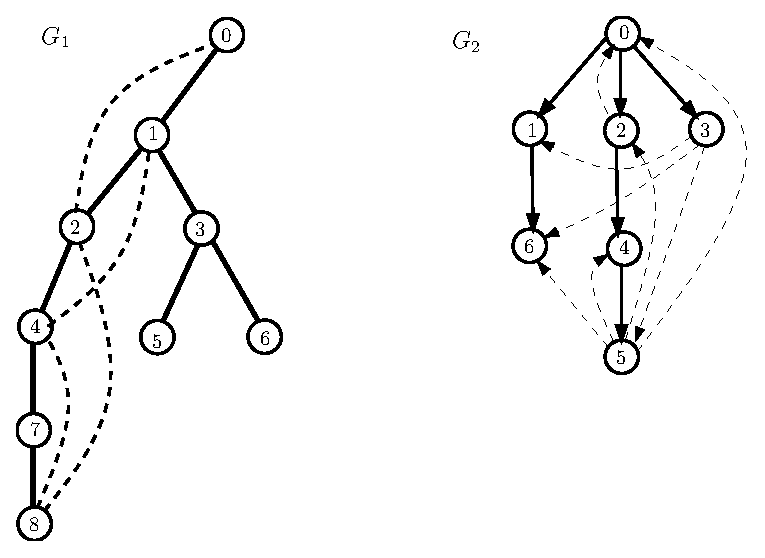
\includegraphics{./figs/graphEx2DFS.eps}}

\caption{DFS trees for $G_1$ and $G_2$, rooted at $0$}

\end{figure}

In the examples above, all nodes were reachable from the root, and so
there is a single search tree in the forest. For general digraphs, this
may not be true. We should distinguish between BFS or DFS originating
from a given node, or just BFS/DFS run on a digraph. The former we call
\algfont{BFSvisit/DFSvisit} (a special case of \algfont{visit}) and the
latter just \algfont{BFS/DFS} (a special case of \algfont{traverse}). The
algorithm \algfont{DFS}, for example, repeatedly chooses a root and runs
\algfont{DFSvisit} from that root, until all nodes have been visited.
Pseudocode for these procedures is given in the next two subsections.

\subsection{Additional discussion of depth-first search}
\label{ss: DFS}

In DFS, the next grey node chosen is the last one to be coloured grey thus far. The data structure for processing grey nodes  in this ``last in, first
out" order is therefore a stack (see Appendix~\ref{app:datastruct} if
necessary for the basic facts about stacks). We may store the nodes in a
stack as they are discovered. So the general \algfont{traverse} and
\algfont{visit} procedures can be replaced by those in
Figure~\ref{fig:DFScode}. Note how the pseudocode for \algfont{visit} has
been altered. We loop through the nodes adjacent to the chosen grey node
$u$, and as soon as we find a white one, we add it to the stack. We also
introduce a variable $time$ and keep track of the time a node was turned
grey, and the time it was turned black, in the arrays $seen, done$.
These will be useful later.

\begin{figure}[htbp]
\label{fig:DFScode}

\Algorithm{dfs}{digraph $G$}{}
{
stack $S$ \\ 

array $colour[n], pred[n], seen[n], done[n]$ \\

\textbf{for} $u \in V(G)$ \textbf{do} \\

\> $colour[u] \gets $ WHITE; $pred[u] \gets $ NULL \\

\textbf{end for}\\

$time \gets 0$ \\

\textbf{for}  $s\in V(G)$ \textbf{do} \\

\> \textbf{if} $colour[s] = $ WHITE \textbf{then} \\

\> \> \algfont{dfsvisit}($s$) \\

\> \textbf{end if}\\

\textbf{end for}\\

\textbf{return} $pred, seen, done$ \\
}


\Algorithm{dfsvisit}{node $s$}{}
{
$colour[s] \gets $ GREY \\

$seen[u] \gets time$; $time \gets time + 1$ \\

S.push($s$) \\

\textbf{while not} S.isempty() \textbf{do} \\

\> $u \gets $ S.peek() \\

\> \textbf{for} each $v$ adjacent to $u$ \textbf{do} \\

\> \>  \textbf{if} $colour[v] = $ WHITE \textbf{then} \\

\> \> \> $colour[v] \gets $ GREY; $pred[v] \gets u$ \\

\> \> \>  $seen[v] \gets time$; $\time \gets \time + 1 $ \\

\> \> \> S.push($v$) \\

\> \> \textbf{end if} \\

\> \textbf{end for} \\

\> S.pop() \\

\> $colour[u] \gets $ BLACK \\

\> $done[u] \gets time$; $time \gets time + 1$ \\

\textbf{end while} \\
}

\caption{Depth-first search.}

\end{figure}

The complexity analysis of DFS is easy. Choosing a grey node $u$ takes
constant time since only the stack pop operation is required. The time
taken to apply the selection rule to a white neighbour is also constant,
since we take the first one found in the for-loop. Our analysis of
\algfont{traverse} shows us that \algfont{DFS} runs in time $\Theta(n + e)$
if adjacency lists are used, and $\Theta(n^2)$ using an adjacency matrix.
In summary, \boldfont{DFS is a linear-time traversal algorithm}.

One nice feature of depth-first search is its recursive nature.  The
relationship between stacks and recursion is, we hope, well known to the
reader. We can replace the \algfont{DFSvisit} procedure in this case by
the recursive version in Figure~\ref{fig:DFSreccode}.

\begin{figure}[htbp]
\label{fig:DFSreccode}

\Algorithm{recDFSvisit}{node $s$}{}
{

$colour[s] \gets $ GREY \\

$seen[s] \gets time$; $time \gets time + 1$ \\

\textbf{for} each $v$ adjacent to $s$ \textbf{do} \\

\> \textbf{if} $colour[v] = $ WHITE \textbf{then} \\

\> \> $pred[v] \gets s$ \\

\> \> \algfont{recDFSvisit}($v$) \\

\> \textbf{end if} \\

\textbf{end for} \\

$colour[s] \gets $ BLACK \\

$done[s] \gets time $; $time \gets time + 1$ \\
}

\caption{DFSvisit --- recursive version}

\end{figure}

We now note a few important facts about depth-first search that are
useful in proving correctness of various algorithms later on. 

\begin{Theorem}
\label{thm:white-path}
The call to \algfont{recDFSvisit} with input $s$ terminates only when all nodes reachable from $s$ via a path of white nodes have been visited. The descendants of $s$ in the DFS forest are precisely these nodes. 
\end{Theorem}

\begin{proof}
 **** FIX *****
\end{proof}


There are not as many possibilities for interleaving of the timestamps as there appear at first sight. In particular, we \boldfont{cannot} have $seen[v] < seen[w] < done[v] < done[w]$. The following theorem explains why.

\begin{Theorem}
\label{thm:DFS-seen-done}
Suppose that we have performed DFS on a digraph $G$, resulting in a search forest $F$. Let $v, w\in V(G)$ and suppose that $seen[v] < seen[w]$. 

\begin{itemize}
\item
If $v$ is an ancestor of $w$ in $F$, then 
$$seen[v] < seen[w] < done[w] < done[v].$$
\item
If $v$ is not an ancestor of $w$ in $F$,
$$seen[v] < done[v]  < seen[w] < done[w].$$

\end{itemize}
\end{Theorem}

\begin{proof} The first part is clear from the recursive formulation of DFS. Now suppose that $v$ is not an ancestor of $w$. Note that $w$ is obviously also not an ancestor of $v$. Let $x$ be the root of the tree of $F$ containing $v$. Then $v\neq x, w\neq x$ and $v$ lives in a subtree that is completely explored before the subtree of $w$ is visited by \algfont{recDFSvisit}.

\end{proof}

All four types of arcs in our search forest classification can arise
with DFS. The different types of non-tree arcs can be easily
distinguished while the algorithm is running. For example, if an arc
$(u, v)$ is explored and $v$ is found to be white, then the arc is a
tree arc; if $v$ is grey then the arc is a back arc, and so on (see Exercise~\ref{ex:DFS-cross-vs-forward}).

We can also perform the classification after the algorithm has
terminated, just by looking at the timestamps $seen$ and $done$ (see Exercise~\ref{ex:DFS-arc-class}).  


\subsection*{Exercises}


\begin{Exercise} 
\label{ex:DFS-all-arcs-occur}
Give examples to show that all four types of arcs can arise when DFS is
run on a digraph.
\end{Exercise}

\begin{Exercise}
\label{ex:DFS-doDFS}

Carry out depth-first search on the digraph with adjacency lists
representation  given below. Classify each arc as tree, forward, back or cross.
\newline
$$
\begin{tabular}{ccccc}
0: & 2 &  & \\
1: & 0 & &\\
2: & 0 & 1&\\
3: & 4 & 5 & 6\\
4: & 5 & &\\
5: & 3 & 4 & 6 \\
6: & 1 & 2 & \\
\end{tabular}
$$
\end{Exercise}


\begin{Exercise}
\label{ex:DFS-cross-vs-forward}
Explain how to determine, at the time when an arc is first explored by
DFS, whether it is a cross arc or a forward arc.
\end{Exercise}



\begin{Exercise}
\label{ex:DFS-arc-class}
Suppose that we have performed DFS on a digraph $G$. Let $(v, w)\in
E(G)$. Show that the following statements are true.
\begin{enumerate}
\romenumi
\item
$(v, w)$ is a tree or forward arc if and only if  
$$seen[v] < seen[w] < done[w] < done[v];$$
\item
$(v, w)$ is a back arc if and only if
$$seen[w] <  seen[v] < done[v] < done[w];$$ 
\item
$(v, w)$ is a cross arc if and only if 
$$seen[w] < done[w]  < seen[v] < done[v].$$
\end{enumerate}

\end{Exercise}

\begin{Exercise}[2002 midterm]
\label{ex:DFS-timestamps}
\item Suppose that DFS is run on a digraph $G$ and the following
timestamps obtained.

\

\begin{tabular}{|c|ccccccc|}
\hline 
$v$ & 0 & 1 & 2 & 3 & 4 & 5 & 6 \\
\hline
$seen[v]$ & 0 & 1 & 2 & 11 & 4 & 3 & 6 \\
\hline
$done[v]$ & 13 & 10 & 9 & 12 & 5 & 8 & 7 \\
\hline
\end{tabular}

\

\begin{enumerate}
\romenumi


\item List all tree arcs, forward arcs, back arcs, and cross arcs in the
DFS forest.

%\answer{1}
%{\fbox{\rule[0mm]{0mm}{20mm} \hspace*{115mm}}}{} 
%\marks{3}
\item 
Suppose that $(6,1)$ is an arc of $G$. Which type of arc 
(tree, forward, back or cross) is it?

%\answer{back}
%{\fbox{\rule[0mm]{0mm}{20mm} \hspace*{115mm}}}{} 
%\marks{1}

\item 
Is it possible for node $2$ to be an ancestor of node $3$ in the DFS
forest?

%\answer{NO}
%{\fbox{\rule[0mm]{0mm}{20mm} \hspace*{115mm}}}{} 
%\marks{2}
\item
Is it possible that $G$ contains an arc $(5,3)$? If so, what type of arc
must it be?

%\answer{NO}
%{\fbox{\rule[0mm]{0mm}{20mm} \hspace*{115mm}}}{} 
%\marks{1}
\item 
Is it possible that $G$ contains an arc $(1,5)$? If so, what type of arc
must it be?

%\answer{YES}
%{\fbox{\rule[0mm]{0mm}{20mm} \hspace*{115mm}}}{} 
%\marks{1}
\end{enumerate}


\end{Exercise}

\begin{Exercise}
\label{ex:DFS-tree-vs-nontree}
Is there a way to distinguish tree arcs from non-tree arcs just by
looking at timestamps after DFS has finished running?
\end{Exercise}



\begin{Exercise}
\label{ex:DFS-graph-no-cross}
Suppose that DFS is run on a graph $G$. Prove that cross edges do not occur.
\end{Exercise}


\begin{Exercise}
\label{ex:DFS-false-conj}
Give an example to show that the following conjecture is \boldfont{not
true}: if $w$ is reachable from $v$ and $seen[v] < seen[w]$ then $w$ is
a descendant of $v$ in the DFS forest.
\end{Exercise}


\begin{Exercise}
\label{ex:DFS-prepostorder}
DFS allows us to give a so-called pre-order and post-order labelling to
a digraph. The pre-order label indicates the order in which the nodes
were turned grey. The post-order label indicates the order in which the
nodes were turned black.

For example, each node of the following tree is labelled with a pair of
integers indicating the pre- and post- orders, respectively, of the
layout.

\smallskip

\centerline{\Ipe{./figs/pre+post.ipe}}

This is obviously strongly related to the values in the arrays $seen,
done$. What is the exact relationship between the two?


\end{Exercise}


\subsection{Additional properties of breadth-first search}

The first-in first-out processing of the grey nodes in BFS is ideally
handled by a queue. In Figure~\ref{fig:BFScode} we present the algorithm
in pseudocode. The timestamps $seen, done$ of DFS are of less use here;
it is more useful to record the number of steps from the root in the
array $level$.

\begin{figure}[hbtp]

\Algorithm{bfs}{digraph $G$; queue $Q$, }{}
{
queue $Q$ \\

array $colour[n], pred[n], d[n]$ \\

\textbf{for} $u \in V(G)$ \textbf{do} \\

\> $colour[u] \gets $ WHITE; $pred[u] \gets $ NULL \\

\textbf{end for}\\

\textbf{for}  $s\in V(G)$ \textbf{do} \\

\> \textbf{if} $colour[s] = $ WHITE \textbf{then} \\

\> \> \algfont{BFSvisit}($s$) \\

\> \textbf{end if}\\

\textbf{end for}\\

\textbf{return} $pred, d$\\
}

\Algorithm{BFSvisit}{node $s$}{}
{
$colour[s] \gets $ GREY; $d[s] \gets 0$ \\

Q.insert($s$) \\

$level \gets 0$ \\

\textbf{while not} Q.isempty() \textbf{do} \\

\> $u \gets $ Q.head() \\

\> $level \gets level + 1$ \\

\> \textbf{for} each $v$ adjacent to $u$ \textbf{do} \\

\> \> \textbf{if} $colour[v] = $ WHITE \textbf{then} \\

\> \> \> $colour[v] \gets $ GREY; $pred[v] \gets u$; $d[v] \gets level$
\\

\> \> \> Q.insert($v$) \\

\> \> \textbf{end if} \\

\> \textbf{end for} \\

\> Q.dequeue() \\

\> $colour[u] \gets $ BLACK \\

\textbf{end while} \\
}

\caption{Breadth-first search pseudocode.}
\label{fig:BFScode}

\end{figure}


A similar analysis to what we did for DFS also holds for BFS: it is also
a linear time traversal algorithm, because the next grey and white node 
can again be chosen in constant time.

It is rather obvious that BFS processes all nodes at distance 1, then
all nodes at distance 2, etc, from the root. The formal proof is below.

\begin{Theorem}
\label{thm:BFSdist}
Suppose we run \algfont{BFS} on a digraph $G$.
Let $v\in V(G)$, and let $r$ be the root of the  search tree containing $v$. Then $d[v] = d(r, v)$.
\end{Theorem}

\begin{proof}Note that since $d[v]$ is the length of a path of tree arcs from $r$ to $v$, we have $d[v] \geq d(r, v)$. We prove the result by induction on the distance. Denote the BFS search forest
by $F$ and let $s$ be the root of a tree in $F$. Then $d[s] = 0 =
d(s, s)$ so the result is true for distance zero. Suppose it is true for
all $v$ for which $d(s, v) < k$ and consider a node $v$ such that $d(s,
v) = k \geq 1$. Choose a shortest path from $s$ to $v$ in $G$ and let
$u$ be the penultimate node in the path. Then $d(s, u) = k - 1$ (it
cannot be less, or it would contradict $d(s, v) = k$; on the other hand
the subpath from $s$ to $u$ must be a shortest path from $s$ to $u$,
otherwise we could find a shorter one from $s$ to $v$). By the inductive
hypothesis, $d[u] = d[s, u] = k - 1$. Now $v$ must be seen after $u$
(otherwise $d[v] < k$, but we know $d[v] \geq d(s, v) = k$). Thus $v$ is seen in the loop through white neighbours of $u$, and so $d[v] = d[u] + 1 = k$. This concludes the proof.

\end{proof}

We can classify arcs, but the answer is not as nice as with DFS.

\begin{Theorem}
\label{thm:BFS-arcclass}
Suppose that we are performing \algfont{BFS} on a digraph $G$. Let $(v,
w)\in E(G)$ and suppose that we have just chosen the grey node $v$. 
Then
\begin{itemize}
\item
if $(v, w)$ is a tree arc then $colour[w] = $ WHITE, $d[w] = d[v] + 1$
\item
if $(v, w)$ is a back arc, then $colour[w] = $ BLACK, $d[w] \leq d[v] - 1$  
\item
There are no forward arcs.
\item
if $(v, w)$ is a cross arc then one of the following holds:
\begin{itemize}
\item $d[w] < d[v] - 1$, and $colour[w] = $ BLACK;
\item $d[w] = d[v]$, and $colour[w] = $ GREY;
\item $d[w] = d[v]$, and $colour[w] = $ BLACK;
\item $d[w] = d[v] - 1$, and $colour[w] = $ GREY;
\item $d[w] = d[v] - 1$, and $colour[w] = $ BLACK.
\end{itemize}

\end{itemize}

\end{Theorem}

\begin{proof}
The arc is added to the tree if and only if $w$ is white. If the arc is
a back arc, then $w$ is an ancestor of $v$; the FIFO queue structure
means $w$ is black before the adjacency list of $v$ is scanned. 

Now suppose that $(x, u)$ is a forward arc. Then since $u$ is a
descendant of $x$ but not a child in the search forest, Theorem~\ref{thm:BFSdist} yields $d[u]
\geq d[x] + 2$. But by the last theorem we have $d[u] = d(s, u) \leq
d(s, x) + 1 = d[x] + 1$, a contradiction. Hence no such arc exists.

A cross arc may join two nodes on the same level, jump up one level, or
jump up more than one level. In the last case, $w$ is already black before $v$ is seen. In the second case, $w$ may be seen before $v$, in which case it is black before $v$ is seen (recall $w$ is not the parent of $v$), or it may be seen after $v$, in which case it is grey when $(v, w)$ is explored. In the first case, $w$ may be seen  $v$ (in which case it is black before $v$ is seen), or $w$ may be seen after $v$ (in which case it is grey when $(v, w)$ is explored).

\end{proof}

In the special case of graphs we can say more.

\begin{Theorem}
\label{thm:BFS-grapharcclass}
Suppose that we have performed \algfont{BFS} on a graph $G$. Let $\{v,
w\}\in E(G)$. Then exactly one of the following conditions holds.

\begin{itemize}
\item
$\{v, w\}$ is a tree edge, $d[v] = d[w] + 1$;
\item 
$\{v, w\}$ is a tree edge, $d[w] = d[v] + 1$;
\item
$\{v, w\}$ is a cross edge, $d[w] = d[v]$;
\item
$\{v, w\}$ is a cross edge, $|d[w] - d[v]| = 1$.

\end{itemize}

\end{Theorem}

\begin{proof}
By Theorem~\ref{thm:BFS-arcclass} there can be no forward edges, hence no back edges. A cross edge may not jump up more than one level, else it would also jump down more than one level, which is impossible by Theorem~\ref{thm:BFSdist}. 

\end{proof}

For a given BFS tree, we can uniquely label the vertices of a digraph based on the time they were first seen. For the graph $G_1$ of Figure~\ref{fig:graphExample2}, we label vertex 0 with 1, vertices \set{1,2} with labels \set{2,3}, vertices \set{3,4,8} with labels \set{4,5,6}, and the last vertex level \set{5,6,7}
with labels \set{7,8,9}. These are indicated in
Figure~\ref{fig:graphEx2-BFS}.


\subsection*{Exercises}


\begin{Exercise}
\label{ex:doBFS}

Carry out \algfont{BFS} on the digraph with adjacency list given below. 
Show the state of the queue after each change in its state.
\newline
$$
\begin{tabular}{ccccc}
0: & 2 &  & \\
1: & 0 & &\\
2: & 0 & 1&\\
3: & 4 & 5 & 6\\
4: & 5 & &\\
5: & 3 & 4 & 6 \\
6: & 1 & 2 & \\
\end{tabular}
$$

\end{Exercise}


\begin{Exercise}
\label{ex:BFS-back-vs-cross}

How can we distinguish between a back and a cross arc when BFS is run on
a digraph?

\end{Exercise}

\begin{Exercise}
\label{ex:BFS-cycle}

Explain how to determine whether the root of a BFS tree is contained in
a cycle, while the algorithm is running. You should find a cycle of
minimum length if it exists.

\end{Exercise}


\section{Priority-first search}
\label{sec:PFS}

Priority-first search is a more sophisticated form of traversal with
many applications. For now, we consider it simply as a common
generalization of breadth-first and depth-first search. Priority-first
search may seem a little abstract compared to the more concrete DFS and
BFS. We shall not need it until Chapter~\ref{ch:weighted}; however
it will be essential then.

The important property is that each grey node has associated with it an
integer \defnfont{key}. The interpretation of the key is of a priority: the
smaller the key, the higher the priority. The rule for selecting a new
grey node is to choose one with smallest key.  

In the simplest form of PFS, the key value is assigned when the node
becomes grey, and never updated subsequently. More generally, the key
may be further updated at other times. We shall see both types in this
book. The second type of PFS is used in optimization problems as we
shall discuss in Chapter~\ref{ch:weighted}. 

The first type of PFS includes both BFS and DFS. In BFS, the key value
of $v$ can be taken as $seen[v]$. Note that this means that a given grey
node can be selected many times --- until it becomes black, in fact, it
will always have minimum key among the grey nodes. By contrast, in DFS
we can take the key value to be $- seen[v]$. Then the last node
seen always has minimum key. It cannot be chosen again until the nodes
seen after it have become black.

The running time of PFS depends mostly on how long it takes to find the
minimum key value, and how long it takes to update the key values.

In the array implementation mentioned above, finding the minimum key
value takes time of order $n$ at each step, so the quantity $a$ is
$\Omega(n)$. Thus a PFS of this type will take time in $\Omega(n^2)$.
This is worse than the $\Theta(n + e)$ we obtain with BFS and DFS using
adjacency lists and a queue or stack respectively. One reason is that a
simple array is not a particularly good data structure for finding the
minimum key. You have already seen a better one in Part I of this book
--- the binary heap. In fact PFS is best described via the priority
queue ADT. *** DESCRIBE PRIORITY QUEUE SOMEWHERE - APPENDIX OR PART 1 *** 

Pseudocode demonstrating the first type of PFS is presented in
Figure~\ref{fig:PFScode}. The subroutine \algfont{setkey} there is the rule for giving the key value when a node is inserted. We do not include any code for \algfont{setkey}.

\begin{figure}
\Algorithm{pfs}{digraph $G$}{}
{
priority queue $Q$\\

array $colour[n], pred[n]$ \\

\textbf{for} $u \in V(G)$ \textbf{do} \\

\> $colour[u] \gets $ WHITE; $pred[u] \gets $ NULL \\

\textbf{end for}\\

\textbf{for}  $s\in V(G)$ \textbf{do} \\

\> \textbf{if} $colour[s] = $ WHITE \textbf{then} \\

\> \> \algfont{BFSvisit}($s$) \\

\> \textbf{end if}\\

\textbf{end for}\\

\textbf{return} $pred$\\
}




\Algorithm{PFSvisit}{node $s$}{}
{
$colour[s] \gets $ GREY \\

Q.\algfont{insert}($s$, \algfont{setkey} $(s)$) \\

\textbf{while not} Q.\algfont{isempty}() \textbf{do} \\

\> $u \gets $ Q.min() \\

\> \textbf{for} each $v$ adjacent to $u$ \textbf{do} \\

\> \>  \textbf{if} $colour[v] = $ WHITE \textbf{then} \\

\> \> \> $colour[v] \gets $ GREY \\

\> \> \> Q.\algfont{insert}($v$, \algfont{setkey} $(v)$) \\

\> \> \textbf{end if} \\

\> \textbf{end for} \\

\> Q.\algfont{deletemin}() \\

\> $colour[u] \gets $ BLACK \\

\textbf{end while} \\
}

\caption{Priority-first search.}
\label{fig:PFScode}

\end{figure}

We proceed to show some applications of BFS and DFS in the following
sections. Applications of PFS will be discussed in
Chapter~\ref{ch:weighted}.

\subsection*{Exercises}

\section{Connectivity}
\label{sec:connectivity}

For many purposes it is useful to know whether a digraph is ``all in one
piece", and if not, to decompose it into pieces. We now formalize these
notions. The situation for graphs is easier than that for digraphs.

\begin{Definition} A graph is \defnfont{connected} if for each pair of 
vertices $u, v\in V(G)$, there is a path between them.

\end{Definition}

In Example~\ref{eg:graphExample} the graph $G_1$ is connected, as is the
underlying graph of $G_2$. 

If a graph is not connected, then it must have more than one ``piece".
More formally, we have the following.

\begin{Theorem}
\label{thm:components}
Let $G$ be a graph. Then $G$ can be uniquely written as a union of
subgraphs $G_i$ with the following properties:
\begin{itemize}
\item each $G_i$ is connected
\item if $i\neq j$, there are no edges from any vertices in $G_i$ to any vertices in $G_j$
\end{itemize}

\end{Theorem}

\begin{proof}
Consider the relation $\sim$ defined on $V(G)$, given by $u\sim v$ if
and only if there is a path joining $u$ and $v$ (in other words, $u$ and
$v$ are each reachable from the other). Then $\sim$ is an equivalence
relation and so induces a partition of $V(G)$ into disjoint subsets. The
subgraphs $G_i$ induced by these subsets have no edges joining them by
definition of $\sim$, and each is connected by definition of $\sim$.
\end{proof}

The subgraphs $G_i$ above are called the \defnfont{connected components}
of the graph $G$. Clearly, a graph is connected if and only if it has
exactly one connected component.

\begin{Example}
\label{eg:components}
The graph obtained by deleting an edge from a triangle has 3 connected components *** do a better one PICTURE ***

\end{Example}

We can determine the connected components of a graph easily by using a
traversal algorithm. The following obvious theorem explains why.

\begin{Theorem}
\label{thm:trav-comps}
Let $G$ be a graph and suppose that DFS or BFS is run on $G$. Then the
connected components of $G$ are precisely the subgraphs spanned by the
trees in the search forest. 
\end{Theorem}

\begin{proof}
The result is true for any traversal procedure, as we have already observed in Theorem~\ref{thm:trav}. The trees of the search forest have no edges joining them, and together they span $G$.
\end{proof}

So we need only run BFS or DFS on the graph, and keep count
of the number of times we choose a root --- this is the number of
components. We can store or print the vertices and edges in each
component as we explore them. Clearly, this gives a linear time algorithm
for determining the components of a graph.

So far it may seem that we have been too detailed in our treatment of 
connectedness. After all the above results are all rather obvious.
However, now consider the situation for digraphs.

The intuition of ``being all in one piece" is not as useful here. In
Example~\ref{eg:graphExample} the graph $G_1$ is connected, as is the
underlying graph of $G_2$. They are ``all in one piece", but not the
same from the point of view of reachability. For example, in digraph
$G_2$, node $2$ is a sink. This motivates the following definition.

\begin{Definition}
A digraph $G$ is \defnfont{strongly connected} if for each pair of nodes $u, v$ of $G$, there is a path in $G$ from $u$ to $v$.
\end{Definition}

\begin{note}
In other words, $u$ and $v$ are each reachable from the other.

Suppose that the underlying graph of $G$ is connected (some authors call
this being \defnfont{weakly connected}), but $G$ is not strongly
connected. Then if $G$ represents a road network, it is possible to get
from any place to any other one, but at least one such route will be
illegal: one must go the wrong way down a one-way street. \end{note}A
strongly connected digraph must contain many cycles: indeed, if $v$ and
$w$ are different nodes, then there is a path from $v$ to $w$ and a path
from $w$ to $v$, so $v$ and $w$ are contained in a cycle. Conversely, if
each pair of nodes is contained in a cycle, then the digraph is clearly
strongly connected.

Again, we can define \defnfont{strongly connected components} in a way that is entirely analogous to component for graphs. The proof above for connected components generalizes to this situation.

\begin{Theorem}
\label{thm:scc}
Let $G=(V, E)$ be a digraph. Then $V$ can be uniquely written as a union of disjoint subsets $V_i$, with corresponding induced subdigraphs $G_i$,  with the following properties:
\begin{itemize}
\item each $G_i$ is strongly connected
\item if $i\neq j$, $v\in G_i, w\in G_j$, and $(v, w) \in E(G)$ then $(w, v) \not\in E(G)$. 
\end{itemize}

\end{Theorem}

\begin{proof}
Consider the relation $\sim$ defined on $V$, given by $u\sim v$ if
and only if there is a path joining $u$ and $v$ and a path joining $v$ and $u$ (in other words, $u$ and $v$ are each reachable from the other). Then $\sim$ is an equivalence relation and so induces a partition of $V$ into disjoint subsets. The subgraphs $G_i$ induced by these subsets satisfy the stated conditions by definition of $\sim$.
\end{proof}



\begin{Example}\label{eg:scc}

A digraph and its three (uniquely determined) strongly connected
components are displayed in Figure~\ref{fig:scc}. Note that there are arcs of the digraph not included in the strongly connected components. 


\end{Example}


\begin{figure}[htbp]
\centerline{\Ipe{./figs/SCC.ipe}}

\caption{A digraph and its strongly connected components.}
\label{fig:scc}
\end{figure}

Note that if the underlying graph of $G$ is connected but $G$ is not
strongly connected, then  there are strong components $C_1$ and $C_2$
such that it is possible to get from $C_1$ to $C_2$ but not from $C_2$
to $C_1$. If $C_1$ and $C_2$ are different strong components, then any
arcs between them must either all point from $C_1$ to $C_2$ or from $C_2$
to $C_1$.  Suppose that we imagine each strong component shrunk to a
single node (so we ignore the internal structure of each component,
but keep the arcs between components). Then in the digraph resulting,
if $v\neq w$ and we can get from $v$ to $w$ then we cannot get from
$w$ to $v$. In other words, no pair of nodes can belong to a cycle,
and hence the digraph has no cycles. See Figure~\ref{fig:sccdecomp}.

\begin{figure}[htbp]
\label{fig:sccdecomp}

\caption{Structure of a digraph in terms of its strong components}
\end{figure}

Note the similarity between this and the search forest decomposition in Figure~\ref{fig:travdecomp}. In that case, if we shrink each search tree to a point, the resulting digraph also has no cycles. 

How to determine the strongly connected components? First we observe
that the previous method for graphs definitely fails (see
Exercise~\ref{ex:DFSfails}). To decide whether a digraph is strongly
connected we could run \algfont{BFSvisit} or \algfont{DFSvisit}
originating from each node in turn and see whether each of the $n$ trees
so generated spans the digraph. However the running time of such an
algorithm is $\Theta(n^2+ne)$.

We can do better by using DFS more cleverly. To see how, we need to
examine the structure of $G$ more closely. If we run DFS once on a
digraph $G$, we create a search forest $F$ with trees $T_1, \dots ,T_m$
say,and corresponding induced subdigraphs $G_1, \dots , G_m$. Each tree
does not necessarily span a single strong component. However, note that
if $x$ is the first node of a given strong component to be visited,
then by Theorem~\ref{thm:white-path}, the entire strong component is a
subtree below $x$. This strong component then clearly lies in the same
tree as $x$.

Let $S_{ij}$ be the $j$th strong component of $G_i$ discovered by
DFS. Then $G$ consists of the subdigraphs $S_{ij}$ with arcs linking
them. Each arc has the property that its tail lies in  a component
with a value of $i$ that is not greater than where its head lives;
if the $i$-values are equal then its tail has a lower value of $j$.
The search begins in $S_{11}$, reaches $S_{12}, S_{13}$, etc, and finishes
exploring these components in the reverse order they were discovered. See
Figure~\ref{fig:scc-alg1}. This picture makes it fairly clear how we
should proceed.

\begin{figure}

\caption{Digraph decomposition with respect to strong components and DFS
trees.}
\label{fig:scc-alg1}
\end{figure}

Consider the last tree $T_m$ of $F$ to be discovered and the first
of its components $S_{m1}$ to be discovered by DFS. This is the strong
component of the root $s$ of $T_m$. No arcs can enter this from any other
$S_{ij}$. So in the reverse digraph $G_r$, no arcs leave $S_{m1}$ for any
other components. Thus performing \algfont{DFSvisit}, this time on $G_r$
with some root in $S_{m1}$ (for example, we can use $s$), will yield a
tree whose span is contained in $S_1$ and hence  exactly equals $S_1$.

Next, perform \algfont{DFSvisit} on $G_r$, starting inside $S_{m2}$ with
some root $y$. Then every other node of $S_{m2}$ is a descendant of $y$,
and the only other nodes reachable from $y$ in $G_r$ were already seen
in the exploration of $G_r$ from $x$. Thus the tree of $y$ spans exactly
$S_{m2}$. Continuing in this manner, we obtain the components $S_{ij}$
in order of increasing $j$ and decreasing $i$.

We have shown that if we can choose the roots for the second DFS
correctly, then we can find all strong components. Now of course we
don't know these components \emph{a priori}, so how do we identify the
roots to choose in the second DFS run?

One answer is as follows: whenever there is a choice for the root of a
new search tree in the second DFS, choose the first node of that strong
component that was found in $F$. At first sight we still don't know what
that node was.  It turns out that the following simple rule works.

\begin{Theorem} \label{thm:scc-alg} 
If the following rule for choosing
roots is used in the algorithm described above, then each tree in the
second search forest spans a strong component of $G$, and all strong
components arise this way.

Rule: use the white node whose finishing time in $F$ was largest.

\end{Theorem}

\begin{proof}
Let $x_{ij}$ be the first node of $S_{ij}$ to be seen in $F$. We shall
show that the $x_{ij}$ are chosen as roots by the rule above, in the
right order (decreasing $i$, increasing $j$). The result then follows
by the remarks above.

Note that if $r\in S_{ij}$ is a root chosen by the given rule, then it
must equal $x_{ij}$, since $x_{ij}$ is an ancestor in $F$ of all nodes
in $S_{ij}$ and hence finished no earlier than $r$ in the first DFS run.

Clearly each strong component is reached in the second search. So we
need to show only that no tree in the second forest contains more than
one strong component. Suppose that one such tree does contain more than
one strong component. Let $S_{ij}$ be the first one seen in the second
DFS run, and let $S_{il}$ be another. We already know that we cannot
have $l > j$, so $l < j$. Then we must have chosen $r=x_{ij}$ as the
root of this tree, and there must be an arc $(u, v)$ of $G_r$ with $u\in
S_{ij}, v\in S_{il}$. But $s=x_{il}$ is still white when $r$ is chosen,
and $s$ was seen before $r$ in $F$. Thus we have $seen[r] > seen[s]$
and $done[r] > done[s]$. Hence $S_{il}$ was explored in $F$ before $r$
(and hence any node of $S_{ij}$) was seen. But since $u$ was reachable
from $s$ via a path of white nodes in $F$, Theorem~\ref{thm:white-path}
gives a contradiction.
\end{proof} 

The above algorithm runs in linear time with adjacency lists, since each
DFS and the creation of the reverse digraph take linear time. We only
need to remember  while performing the first DFS to store the nodes in
an array in order of finishing time. Otherwise, even if we had stored the
$done$ array, we would need to find an order statistic of that array $n$
times, which would take time in $\Theta(n\log n)$.


\subsection*{Exercises}

\begin{Exercise}
\label{ex:DFSfails}

Give an example to show that a single use of DFS does not in general find the strongly connected components of a digraph.
\end{Exercise}

\begin{Exercise}
\label{ex:dolinscc}

Carry out the above  algorithm by hand on the digraph of
Example~\ref{eg:scc} and verify that the components given there are
correct. Then run it again on the reverse digraph and verify that the
answers are the same.
\end{Exercise}


\section{Cycles}
\label{sec:cycles}

In this section, we cover three varied topics concerning cycles.

\subsection{Acyclic graphs and DAGs}
\label{subsec:dag}

A digraph without cycles is commonly called a \defnfont{DAG}, an
abbreviation for \textbf{d}irected \textbf{a}cyclic
\textbf{g}raph. It is much easier for a digraph to be a
DAG than for its underlying graph to be acyclic. 

To determine whether a digraph is acyclic, we can use DFS.  In a cycle, 
one must eventually reach a node that points to one that has been seen
before. In other words, we will detect a back arc. The details and proof
that this works now follow.

\begin{Theorem}
\label{thm:DAG}
Suppose that DFS is run on a digraph $G$. Then $G$ is acyclic if and
only if there are no back arcs.
\end{Theorem}

\begin{proof}
Suppose that we run DFS on $G$. Note that if there is a
back arc $(v, u)$, then $u$ and $v$ belong to the same tree $T$, with
root $s$ say. Then there is a path from $s$ to $u$, and there is a path
from $u$ to $v$ by definition of back arc. Adding the arc $(v, u)$ gives
a cycle. 

Conversely, if there is a cycle $v_0\, v_1\, \dots \, v_n\, v_0$, we may
suppose without loss of generality that $v_0$ is the first node of the
cycle  visited by the DFS algorithm. We claim that $(v_n, v_0)$ is a
back arc. To see why this is true, note that since $v_0$ is linked to
$v_n$ via a path of white nodes, $v_n$ is a descendant of $v_0$ in the
DFS forest by Theorem~\ref{thm:white-path}. 
\end{proof}

This shows correctness of our algorithm for determining acyclicity. What
the time complexity of this algorithm?  Since the back arc can be
detected while DFS is running, but it may not be found until the last
step, the best bound we have is $\Theta(n+e)$. 

The above algorithm of course works for graphs, but there
is another solution in this case. It is not hard to show (see
Appendix~\ref{app:mathfacts}) that a connected graph $G$ is acyclic if and
only if $|V(G)| = 1 + |E(G)|$, and this occurs if and only if $G$ is a
(free) tree. We get the following linear time algorithm for determining
whether a graph $G$ is acyclic. Simply run a graph traversal such as
BFS or DFS, and count the number $k$ of trees in the search forest. Then
just check whether $|V(G)| = k + |E(G)|$.

\subsection{The girth of a graph}
\label{subssec:girth}

In a communication network, small cycles are often something to be
avoided; they can slow down message propagation. The length of the
smallest cycle in a graph is an important quantity.

\begin{Definition}

For a graph (with a cycle), the length of the shortest cycle is called
the \defnfont{girth} of the graph. If the graph has no cycles then the
girth is undefined but may be viewed as $+\infty$.

\end{Definition}

\begin{note} For a digraph we use the term girth for its underlying
graph and the (maybe non-standard) term \defnfont{directed girth} for
the length of the smallest directed cycle.

\end{note}

\begin{Example}
\label{eg:cycles}
In Figure~\ref{fig:cycle} are three (di)graphs.  The first has no cycles (it is a free tree), the second is a DAG, and the third has  girth 4.
\end{Example}

\begin{figure}
\label{fig:cycle}

\centerline{\Ipe{./figs/graphEx3.ipe}}
\caption{Some (di)graphs with different cycle behaviour}
\end{figure}

How to compute the girth of a graph? Here is an algorithm for finding
the length of a shortest cycle containing a given vertex $v$ in a graph
$G$. Perform \algfont{BFSvisit}. If we meet a grey neighbour (that is,
we are exploring edge $\{x, y\}$ from $x$ and we find that $y$ is already
grey), continue only to the end of the current level and then stop. For
each edge $\set{x, y}$ as above on this level, if $v$ is the lowest
common ancestor of $x$ and $y$ in the BFS tree, then there is a cycle
containing $x, y, v$ of length $l:=d(x) + d(y) + 1$. Report the minimum
value of $l$ obtained along the current level.

\begin{Theorem}
\label{thm:BFS-cycle} 

The above algorithm is correct.

\end{Theorem}


\begin{proof}

Suppose that we arrive at vertex $x$, $d(x) = k$, and we have just
encountered a grey neighbour $y$. Then $d[y] = d[x] + 1$ or $d[y] = d[x]$
(note that $d[x] = d[y] + 1$ is ruled out because then $x$ would be a
child of $y$ and $y$ would be black). This means that there is definitely
a cycle containing $x, y$ and $z$, where $z$ is the lowest common ancestor
of $x$ and $y$ in the BFS tree. Note that $z\neq x, z\neq y$ since neither
$x$ nor $y$ is an ancestor of the other. The cycle consists of the tree
edges from $z$ to $x$, the cross edge $\set{x,y}$ and the tree edges
from $z$ to $y$. The length of the cycle is $l:=d[x] + d[y] - 2 d[z] + 1$.

Conversely, let $C$ be any cycle and let $z$ be the first vertex of
the cycle reached by the search. Let $x$ and $y$ be two vertices in $C$
whose distance  from $z$ is greatest, with $d[x] \leq d[y]$. Then the
lowest common ancestor of  $x$ and $y$ is exactly $z$, and the cycle
found in the first paragraph is exactly $C$.

The vertex $v$ belongs to the cycle $C$ if and only if $v = z$. The
length of the cycle is $2k+1$ if $d[x] = d[y]$ and $2k+2$ if $d[y] =
d[x] - 1$. The minimum length of any cycle containing $v$ found after
this is $2(k+1) + 1 = 2k+3$, so no better cycle can be found after the
current level $k$ is explored.

\end{proof}

\begin{note}

An easy-to-implement DFS idea may not work properly. For example,
the DFS tree originating from vertex $0$ of the third graph of
Example~\ref{eg:cycles} finds only $6$-cycles with the back edges (even
though a $4$-cycle exists using two of the back edges).

\end{note}

To compute the girth of a graph, we can simply run the above algorithm
from each vertex in turn, and take the minimum cycle length achieved.

\subsection{Bipartite graphs}
\label{subsec:bipartite}

Many graphs in applications have two different types of nodes, and no
relations between nodes of the same type (this is a model of sexually
reproducing organisms, for example).

\begin{Definition}

A graph $G$ is \defnfont{bipartite} if $V(G)$  can be partitioned into
two nonempty disjoint subsets $V_0, V_1$ such that each edge of $G$
has one endpoint in $V_0$ and one in $V_1$.

\end{Definition}

\begin{Example}

**** PICTURE ****

\end{Example}

Showing that a graph is bipartite can be done by exhibiting a
\defnfont{bipartition} (a partition into two subsets as in the
definition). Of course finding such a bipartition may not be easy. Showing
a graph is not bipartite seems even harder. In each case, we certainly
do not want to have to try all possible partitions of $V$ into two
subsets! There is a better way.

\begin{Definition}
Let $k$ be a positive integer. A graph $G$ has a \defnfont{$k$-colouring}
if $V(G)$ can be partitioned into $k$ nonempty disjoint subsets such
that each edge of $G$ joins two vertices in different subsets.
\end{Definition}

\begin{Example}

*** PICTURE ****

\end{Example}

\begin{Theorem} The following conditions on a graph $G$ are equivalent.
\begin{itemize}
\item
$G$ is bipartite;
\item
$G$ has a $2$-colouring;
\item
$G$ does not contain an odd length cycle.
\end{itemize}
\end{Theorem}

\begin{proof} 

Given a bipartition, use the same subsets to get a $2$-colouring, and
vice versa. This shows the equivalence of the first two conditions. Now
suppose $G$ is bipartite.  A cycle must have even length, since the start
and end vertices must have the same colour. Finally suppose that $G$
has no odd length cycle. A $2$-colouring is obtained as follows. Perform
BFS and assign each vertex at level $i$ the ``colour" $i \mod 2$. If we
can complete this procedure, then by definition each vertex goes from
a vertex of one colour to one of another colour. The only problem could
be if we tried to assign a colour to a node $v$ that was adjacent to a
node $w$ of the same colour at the same level $k$. But then a cycle of
length $2k+1$ is created.
\end{proof}

It is now easy to see that we may use the method in the proof above
to detect an odd length cycle if it exists, and otherwise produce a
$2$-colouring of $G$. This of course runs in linear time.


\subsection*{Exercises}


\begin{Exercise}
\label{ex:DAG-vs-tree}
Give an example of a DAG whose underlying graph contains a cycle. Make
your example as small as possible.

\end{Exercise}

\begin{Exercise}
\label{ex:DAG-sink}
Prove that every DAG must have at least one source and at least one sink.
\end{Exercise}


\begin{Exercise}
\label{ex:shortest-cycle-thm}

Give an example to show that in the shortest cycle algorithm, if we
do not continue to the end of the level, but terminate when the first
cycle is found, we may find a cycle whose length is one more than the
shortest possible.

\end{Exercise}

\begin{Exercise}
\label{ex:shortest-cycle-runtime}

What is the time complexity of the shortest cycle algorithm?

\end{Exercise}

\begin{Exercise}
\label{ex:do2col}

The \defnfont{$n$-cube} is a graph on $2^n$ vertices, each labelled by
a different bit vector of length $n$. If $\mathbf{v} = (v_0, \dots ,
v_{n-1}$ and $\mathbf{w} = (w_0, \dots , w_{n-1})$ are such bit vectors,
then there is an edge between the vertex labelled $\mathbf{v}$ and a
vertex labelled $\mathbf{w}$ if and only if all components of the two
vectors, except exactly one of them, are the same.  For which values of
$n$ is the $n$-cube bipartite?
\end{Exercise}

\section{Topological Sorting}
\label{sec:topsort}

In this section we show how to arrange the nodes of an acyclic digraph
into a topological or precedence order.  Many computer science
applications require us to find precedences (or dependencies) among
events, such as a compiler evaluating sub-expressions of an expression
like that shown in Figure~\ref{fig:prec}.

\begin{figure}[hbtp]
\label{fig:prec}


\centerline{\Ipe{./figs/precedence.ipe}}

\caption{Digraph describing structure of an arithmetic expression}
\end{figure}

Here the compiler would need to compute, for example, both $(a+b)$ and
$c$ before it can compute $c-(a+b)$.



\begin{Definition}

Let $G$ be a DAG. A \defnfont{topological sort} of $G$ is a linear
ordering of all its vertices such that if $G$ contains an arc $(u,v)$,
then $u$ appears before $v$ in the ordering.

\end{Definition}

\begin{note}
Clearly if the digraph contains a cycle, it is not possible to find such
a linear ordering, so the condition that $G$ be a DAG is necessary. If a
topological sort exists, then it is possible to draw a picture  of $G$
with all nodes in a straight line, and the arcs ``pointing the same
way".
\end{note}

The term topological sort comes from the study of partial orders and is
sometimes called a \defnfont{topological order} or \defnfont{linear
order}.  For our previous arithmetic expression example, a linear
order of the sub-expression DAG gives us an order (actually the reverse
of the order) where we can safely evaluate the expression.

\begin{Example}
\label{eg:toporder}

In Figure~\ref{fig:toporder} we list three DAGs and possible topological
orders for each. Note that adding more arcs to a DAG  reduces the number
of topological orders it has.  This is because each arc $(u,v)$ forces
$u$ to occur before $v$, which restricts the number of valid permutations
of the vertices.

\end{Example}


\begin{figure}

\label{fig:toporder}



\centerline{\Ipe{./figs/graphEx4.ipe}}

\caption{Topological orders of some DAGs}
\end{figure}

Observe that many DAGs have more than one possible topological order. 
The algorithms for computing \boldfont{all} of these possible orders are
more advanced than what we have time or space for here. We show how to
compute one such order, however.

It turns out that one valid topological order is simply the reverse of
the DFS finishing times.

\begin{Theorem}
Let $G$ be a DAG. Then listing the nodes in reverse order of DFS
finishing times yields a topological order of $G$.
\end{Theorem}

\begin{proof} 
Consider any arc $(u,v)\in E(G)$. Since $G$ is a DAG,
the arc is not a back arc by Theorem~\ref{thm:DAG}. In the other three
cases, Exercise~\ref{ex:DFS-arc-class} shows that $done[u] > done[v]$,
which means $u$ comes before $v$ in the alleged topological order.

\end{proof}


\subsection*{Exercises}


\begin{Exercise}
\label{ex:sillytopsort}
Show that the following method for topologically sorting a DAG does not work in general: print the nodes in order of visiting time.

\end{Exercise}

\begin{Exercise} 
\label{ex:profP}

Professor P has the following information taped to his mirror, to help
him to get dressed in the morning.

Socks before shoes; underwear before trousers; trousers before belt;
trousers before shoes; shirt before glasses; shirt before tie; tie
before jacket; shirt before hat; shirt before belt.

Find an acceptable order of dressing for Professor P.

\end{Exercise}



\begin{Exercise}
\label{ex:zero-indeg}
Prove correctness of the following algorithm (\defnfont{zero-indegree sorting} for topologically sorting a DAG $G$. Choose a source node, write it, and delete it from $G$. Repeat this procedure. The order of writing of the nodes gives a topological order. Exercise~\ref{ex:DAG-sink} may be helpful.

\end{Exercise}


\begin{Exercise}
\label{ex:zero-indeg-runtime}

What is the time complexity of zero-indegree sort? 
\end{Exercise}